\documentclass[10pt,a4paper]{article}\usepackage[]{graphicx}\usepackage[]{color}
%% maxwidth is the original width if it is less than linewidth
%% otherwise use linewidth (to make sure the graphics do not exceed the margin)
\makeatletter
\def\maxwidth{ %
  \ifdim\Gin@nat@width>\linewidth
    \linewidth
  \else
    \Gin@nat@width
  \fi
}
\makeatother

\definecolor{fgcolor}{rgb}{0, 0, 0}
\newcommand{\hlnum}[1]{\textcolor[rgb]{0.533,0,0.133}{#1}}%
\newcommand{\hlstr}[1]{\textcolor[rgb]{0.667,0.267,0}{#1}}%
\newcommand{\hlcom}[1]{\textcolor[rgb]{1,0.533,0}{#1}}%
\newcommand{\hlopt}[1]{\textcolor[rgb]{0,0,0}{\textbf{#1}}}%
\newcommand{\hlstd}[1]{\textcolor[rgb]{0,0,0}{#1}}%
\newcommand{\hlkwa}[1]{\textcolor[rgb]{0.4,0.067,0.067}{\textbf{#1}}}%
\newcommand{\hlkwb}[1]{\textcolor[rgb]{0,0,0.4}{\textbf{#1}}}%
\newcommand{\hlkwc}[1]{\textcolor[rgb]{0,0,0.4}{#1}}%
\newcommand{\hlkwd}[1]{\textcolor[rgb]{0,0.267,0.4}{#1}}%

\usepackage{framed}
\makeatletter
\newenvironment{kframe}{%
 \def\at@end@of@kframe{}%
 \ifinner\ifhmode%
  \def\at@end@of@kframe{\end{minipage}}%
  \begin{minipage}{\columnwidth}%
 \fi\fi%
 \def\FrameCommand##1{\hskip\@totalleftmargin \hskip-\fboxsep
 \colorbox{shadecolor}{##1}\hskip-\fboxsep
     % There is no \\@totalrightmargin, so:
     \hskip-\linewidth \hskip-\@totalleftmargin \hskip\columnwidth}%
 \MakeFramed {\advance\hsize-\width
   \@totalleftmargin\z@ \linewidth\hsize
   \@setminipage}}%
 {\par\unskip\endMakeFramed%
 \at@end@of@kframe}
\makeatother

\definecolor{shadecolor}{rgb}{.97, .97, .97}
\definecolor{messagecolor}{rgb}{0, 0, 0}
\definecolor{warningcolor}{rgb}{1, 0, 1}
\definecolor{errorcolor}{rgb}{1, 0, 0}
\newenvironment{knitrout}{}{} % an empty environment to be redefined in TeX

\usepackage{alltt}
% \usepackage{Sweave} 
\usepackage{natbib}
\usepackage{graphics}
\usepackage{amsmath}
\usepackage{indentfirst}
\usepackage{hanging}
%\usepackage{zi4}
%\usepackage[utf8]{inputenc}
\usepackage{hyperref}
\usepackage[T1]{fontenc}
\DeclareGraphicsExtensions{.png,.pdf,.jpg}
% !Rnw weave = Sweave
\IfFileExists{upquote.sty}{\usepackage{upquote}}{}
\begin{document}
% \SweaveOpts{concordance=TRUE}

%\VignetteIndexEntry{Species distribution modeling with three-step pseudo--absences}
%\VignetteDepends{mopa,sp,raster,earth}
%\VignetteKeyword{spatial}

%\newcommand{\super}[1]{\ensuremath{^{\textrm{#1}}}}
%\newcommand{\sub}[1]{\ensuremath{_{\textrm{#1}}}}
%\newcommand{\R}{{\normalfont\textsf{R }}{}}

% \SweaveOpts{pdf=TRUE, png=TRUE}
% \SweaveOpts{resolution=100}
% \SweaveOpts{keep.source=TRUE}








\title{mopa (MOdelling with Pseudo Absences): A framework for species distribution modelling with
improved pseudo-absence generation}
\author{M. Iturbide et al.}

\tableofcontents

\maketitle


\section{Introduction}
This is a tutorial containing a full worked example of species distribution modelling using the RSEP method and the three-step methods (TS and TSKM methods) for pseudo-absence generation presented in Iturbide et al., 2015, combining environmental profiling and spatial extent restriction of the background (see Fig. 2 in the cited article). We illustrate the steps followed to produce some of the analyses presented in the article using the R package \texttt{mopa} (MOdelling Pseudo Absences). \\



--> NOTE: Most functions presented are implemented in \texttt{mopa}. In the few cases in which functions from other packages are used, the package name is always explicitly indicated.


\subsection{Installing the mopa package}

The \texttt{mopa} package is available on GitHub. The stable release for the package is on the \texttt{master} branch. 

We recommend the \texttt{devtools} package to download and install \texttt{mopa} directly from the stable branch of the repository:

\begin{knitrout}
\definecolor{shadecolor}{rgb}{0.965, 0.965, 0.965}\color{fgcolor}\begin{kframe}
\begin{alltt}
\hlkwa{if} \hlstd{(}\hlopt{!}\hlkwd{require}\hlstd{(devtools))} \hlkwd{install.packages}\hlstd{(}\hlstr{"devtools"}\hlstd{)}
\hlstd{devtools}\hlopt{::}\hlkwd{install_git}\hlstd{(}\hlstr{"https://github.com/SantanderMetGroup/
                      mopa.git"}\hlstd{)}
\end{alltt}
\end{kframe}
\end{knitrout}

Once installed, we load the package:

\begin{knitrout}
\definecolor{shadecolor}{rgb}{0.965, 0.965, 0.965}\color{fgcolor}\begin{kframe}
\begin{alltt}
\hlkwd{library}\hlstd{(mopa)}
\end{alltt}


{\ttfamily\noindent\itshape\color{messagecolor}{\#\# Loading required package: raster\\\#\# Loading required package: sp}}\end{kframe}
\end{knitrout}

\section{Modelling steps}
\subsection{Data pre-processing}

In Iturbide et al., 2015, we indicate the adequacy of using different ecotypes for modelling species distributions. Thus, functions in the \texttt{mopa} package are intended to deal with more than one group of presences simultaneously. In this example, we use a \texttt{list} of 2 different Oak haplotypes (H11 and H5, see Table 1 in the manuscript), but the same steps may be followed in a joint analysis of multiple species. Of course, the most typical case (i.e., dealing with with a single group of species) can be also easily accomplished by providing a \texttt{data.frame}. 

The data set of species in this example is \texttt{Oak\_phylo2} and is provided with the \texttt{mopa} package. This is a modified subset of the \textit{Quercus sp Europe Petit 2002} database (Petit et al., 2002b), which is available in the \textit{Georeferenced Database of Genetic Diversity} or (GD)$^{2}$. To aid in map representation, a dataset called \texttt{wrld} containing a World map is also included in the package.



\begin{knitrout}
\definecolor{shadecolor}{rgb}{0.965, 0.965, 0.965}\color{fgcolor}\begin{kframe}
\begin{alltt}
\hlcom{# Load map and Oak data}
\hlkwd{data}\hlstd{(wrld)}
\hlkwd{data}\hlstd{(Oak_phylo2)}
\hlcom{# Map }
\hlkwd{plot}\hlstd{(wrld,} \hlkwc{asp} \hlstd{=} \hlnum{1}\hlstd{,} \hlkwc{xlim}\hlstd{=} \hlkwd{c}\hlstd{(}\hlopt{-}\hlnum{10}\hlstd{,}\hlnum{50}\hlstd{),} \hlkwc{ylim}\hlstd{=}\hlkwd{c}\hlstd{(}\hlnum{40}\hlstd{,}\hlnum{60}\hlstd{))}
\hlkwa{for} \hlstd{(i} \hlkwa{in} \hlnum{1}\hlopt{:}\hlkwd{length}\hlstd{(Oak_phylo2)) \{}
  \hlkwd{points}\hlstd{(Oak_phylo2[[i]],} \hlkwc{pch} \hlstd{=} \hlstr{"*"}\hlstd{,}
         \hlkwc{cex} \hlstd{=} \hlnum{0.5}\hlstd{,} \hlkwc{col} \hlstd{=} \hlkwd{colors}\hlstd{()[i}\hlopt{*}\hlnum{50}\hlstd{])}
\hlstd{\}}
\end{alltt}
\end{kframe}

{\centering 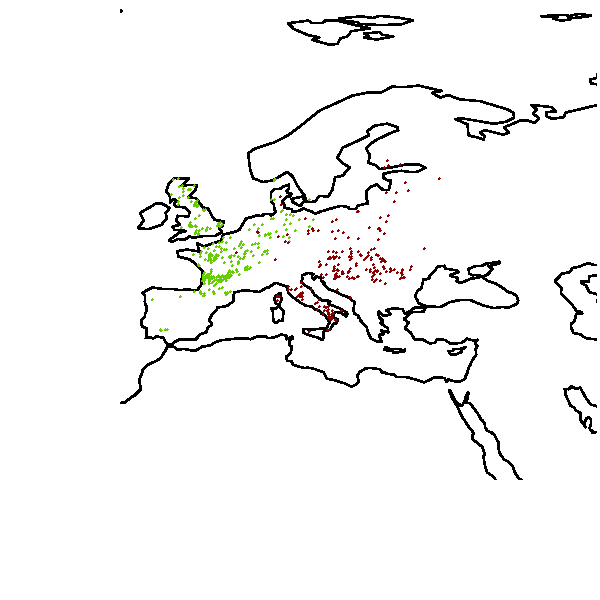
\includegraphics[width=\maxwidth]{figure/graphics-mopa2-1} 

}



\end{knitrout}

Predictor variables are typically stored in raster files. The different raster layers can be efficiently handled in R using the utilities of the \texttt{raster} package. \texttt{mopa} uses as input this type of raster objects. In particular, multiple layers can be arranged in a collection of \texttt{RasterLayers} objects called a \texttt{RasterStack} (see \texttt{?raster::raster} for more information on \texttt{raster} objects). 


\begin{knitrout}
\definecolor{shadecolor}{rgb}{0.965, 0.965, 0.965}\color{fgcolor}\begin{kframe}
\begin{alltt}
\hlcom{# RatserStack of environmental variables}
\hlkwd{data}\hlstd{(biostack)}
\hlkwd{plot}\hlstd{(biostack)}
\end{alltt}
\end{kframe}

{\centering 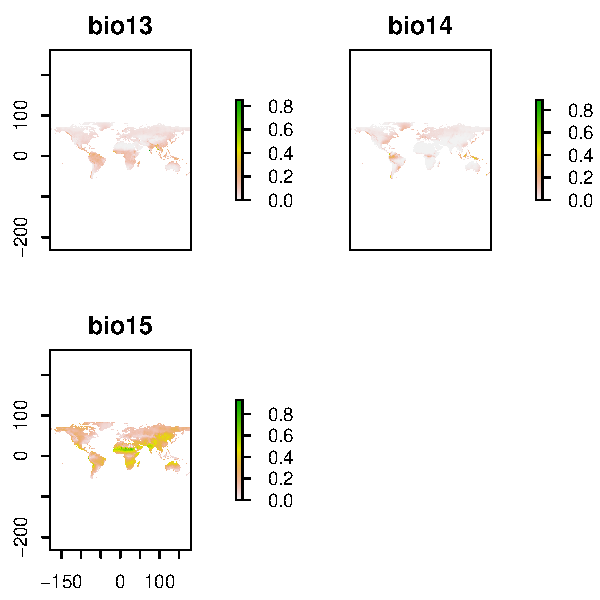
\includegraphics[width=\maxwidth]{figure/graphics-mopa3-1} 

}



\end{knitrout}

The regularly distributed grid points covering the continental area can be created with functions from the \texttt{raster} and \texttt{sp} packages as follows:

\begin{knitrout}
\definecolor{shadecolor}{rgb}{0.965, 0.965, 0.965}\color{fgcolor}\begin{kframe}
\begin{alltt}
\hlcom{# Extract raster values at grid coordinates}
\hlstd{ac} \hlkwb{<-} \hlkwd{xyFromCell}\hlstd{(biostack[[}\hlnum{1}\hlstd{]],} \hlnum{1}\hlopt{:}\hlkwd{ncell}\hlstd{(biostack[[}\hlnum{1}\hlstd{]]))}
\hlstd{ex} \hlkwb{<-} \hlkwd{extract}\hlstd{(biostack[[}\hlnum{1}\hlstd{]], ac)}
\hlcom{# Convert to a Spatial object and define projection}
\hlstd{sp_grid} \hlkwb{<-} \hlkwd{SpatialPoints}\hlstd{(ac[}\hlopt{-}\hlkwd{which}\hlstd{(}\hlkwd{is.na}\hlstd{(ex)), ])}
\hlkwd{projection}\hlstd{(sp_grid)} \hlkwb{<-} \hlkwd{CRS}\hlstd{(}\hlstr{"+proj=longlat +init=epsg:4326"}\hlstd{)}
\end{alltt}
\end{kframe}
\end{knitrout}

For ease of use, the previous steps can be skipped, as the \texttt{sp\_grid} object is already included in the \texttt{mopa} package, covering the whole world at 10 km resolution.

\begin{knitrout}
\definecolor{shadecolor}{rgb}{0.965, 0.965, 0.965}\color{fgcolor}\begin{kframe}
\begin{alltt}
\hlkwd{data}\hlstd{(sp_grid)}
\end{alltt}
\end{kframe}
\end{knitrout}

Function \texttt{boundingCoords} creates a matrix of bounding coordinates around the known presence localities of the target species. In this case, since the \texttt{Oak\_phylo2} list contains two groups of points (one for each haplotype considered), a list of two matrices is created.

\begin{knitrout}
\definecolor{shadecolor}{rgb}{0.965, 0.965, 0.965}\color{fgcolor}\begin{kframe}
\begin{alltt}
 \hlstd{oak.extension} \hlkwb{<-} \hlkwd{boundingCoords}\hlstd{(}\hlkwc{xy} \hlstd{= Oak_phylo2)}
\end{alltt}
\end{kframe}
\end{knitrout}

Function \texttt{delimit} creates a rectangular polygon shape from the bounding coordinates and does the intersection of the background points. A \texttt{list} with two objects is obtained: (1) \texttt{bbs}: polygon shape of the bounding boxes and (2) \texttt{bbs.grid}: a list of data frames of the background point grid limited by the bounding coordinates.


\begin{knitrout}
\definecolor{shadecolor}{rgb}{0.965, 0.965, 0.965}\color{fgcolor}\begin{kframe}
\begin{alltt}
\hlstd{box.grid} \hlkwb{<-} \hlkwd{delimit}\hlstd{(}\hlkwc{bounding.coords} \hlstd{= oak.extension,}
                    \hlkwc{grid} \hlstd{= sp_grid,}
                    \hlkwc{names} \hlstd{=} \hlkwd{names}\hlstd{(Oak_phylo2))}
\hlcom{# Plot presences and bounding boxes}
\hlkwd{plot}\hlstd{(box.grid}\hlopt{$}\hlstd{bbs,} \hlkwc{asp} \hlstd{=} \hlnum{1}\hlstd{)}
\hlkwa{for} \hlstd{(i} \hlkwa{in} \hlnum{1}\hlopt{:}\hlkwd{length}\hlstd{(Oak_phylo2))\{}
  \hlkwd{points}\hlstd{(Oak_phylo2[[i]],} \hlkwc{col} \hlstd{=} \hlkwd{colors}\hlstd{()[i}\hlopt{*}\hlnum{50}\hlstd{])}
\hlstd{\}}
\end{alltt}
\end{kframe}

{\centering 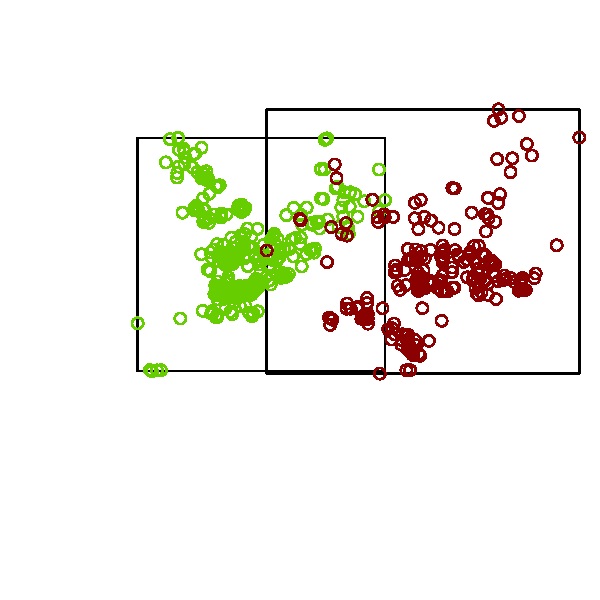
\includegraphics[width=\maxwidth]{figure/graphics-mopa6-1} 

}



\end{knitrout}


\subsection{Three--step pseudo--absences generation}

In this section we illustrate the steps followed to generate pseudo-absences following the RSEP, TS and TSKM procedures described in the manuscript. 

\subsubsection{STEP1: environmental profiling}

The first step is the selection of the environmentally unsuitable areas using a presence-only algorithm. In \texttt{mopa} this is done using a support vector machine-based algorithm that performs a preliminary binary classification of the study region (suitable/unsuitable) using as input the environmental conditions of the presence localities. This is done by function \texttt{OCSVMprofiling} which runs the one-class support vector machine algorithm (OCSVM) for each Oak group of the example:

\begin{knitrout}
\definecolor{shadecolor}{rgb}{0.965, 0.965, 0.965}\color{fgcolor}\begin{kframe}
\begin{alltt}
\hlstd{unsuitable.bg} \hlkwb{<-}\hlkwd{OCSVMprofiling}\hlstd{(}\hlkwc{xy} \hlstd{= Oak_phylo2,}
                               \hlkwc{varstack} \hlstd{= biostack,}
                               \hlkwc{bbs.grid} \hlstd{= box.grid}\hlopt{$}\hlstd{bbs.grid)}
\hlcom{# Plot areas predicted as suitable (presence) and unsuitable }
\hlcom{# (absence) for group H11}
\hlkwd{plot}\hlstd{(unsuitable.bg}\hlopt{$}\hlstd{absence}\hlopt{$}\hlstd{H11,} \hlkwc{pch} \hlstd{=} \hlstr{"*"}\hlstd{,} \hlkwc{asp} \hlstd{=} \hlnum{1}\hlstd{)}
\hlkwd{points}\hlstd{(unsuitable.bg}\hlopt{$}\hlstd{presence}\hlopt{$}\hlstd{H11,} \hlkwc{pch} \hlstd{=} \hlstr{"*"}\hlstd{,} \hlkwc{col} \hlstd{=} \hlstr{"pink2"}\hlstd{)}
\end{alltt}
\end{kframe}

{\centering 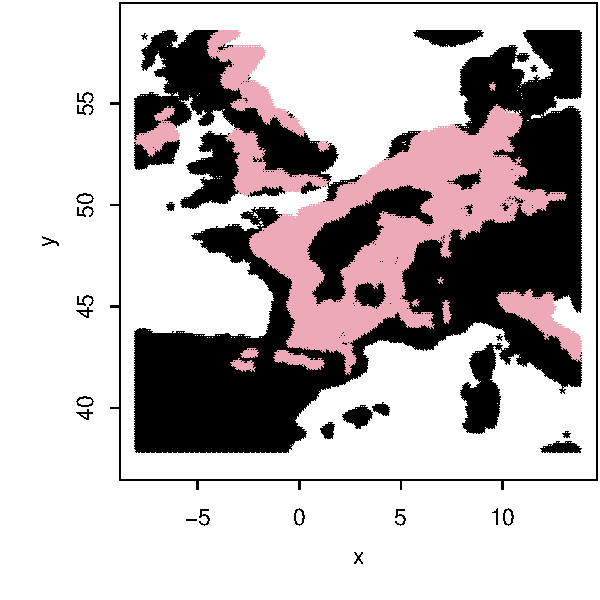
\includegraphics[width=\maxwidth]{figure/graphics-mopa7-1} 

}



\end{knitrout}

If the RSEP method (as described in Iturbide et al., 2015) is selected for pseudo-absence data generation, only the first step is needed, thus, at this point we can create random pseudo-absences in the unsuitable background and perform SDM. The same functions as in the TS and TSKM methods might be used for this purpose, these are \texttt{PseudoAbsences} and \texttt{allModeling}, which are detailed in the section below (STEP2).

\begin{knitrout}
\definecolor{shadecolor}{rgb}{0.965, 0.965, 0.965}\color{fgcolor}\begin{kframe}
\begin{alltt}
\hlcom{# Pseudo--absences are generated at random, in equal number }
\hlcom{# to presences (prevalence) and keeping a 10 km distance to }
\hlcom{# presences (exclusion buffer)}
\hlstd{rsep_random} \hlkwb{<-}\hlkwd{PseudoAbsences}\hlstd{(}\hlkwc{xy} \hlstd{= Oak_phylo2,}
                             \hlkwc{bg.grids} \hlstd{= unsuitable.bg}\hlopt{$}\hlstd{absence,}
                             \hlkwc{exclusion.buffer} \hlstd{=} \hlnum{0.083}\hlstd{,}
                             \hlkwc{prevalence} \hlstd{=} \hlnum{0.5}\hlstd{,} \hlkwc{kmeans} \hlstd{=} \hlnum{FALSE}\hlstd{)}

\hlcom{# Bind presences and absences before modelling}
\hlstd{presausRSEP} \hlkwb{<-} \hlkwd{list}\hlstd{()}
\hlkwa{for} \hlstd{(i} \hlkwa{in} \hlnum{1}\hlopt{:}\hlkwd{length}\hlstd{(Oak_phylo2))\{}
  \hlstd{xyp} \hlkwb{<-} \hlkwd{cbind}\hlstd{(Oak_phylo2[[i]],} \hlkwd{rep}\hlstd{(}\hlnum{1}\hlstd{,} \hlkwd{nrow}\hlstd{(Oak_phylo2[[i]])))}
  \hlstd{xya} \hlkwb{<-} \hlkwd{cbind}\hlstd{(rsep_random[[i]],} \hlkwd{rep}\hlstd{(}\hlnum{0}\hlstd{,} \hlkwd{nrow}\hlstd{(rsep_random[[i]])))}
  \hlkwd{colnames}\hlstd{(xyp)} \hlkwb{<-}  \hlkwd{c}\hlstd{(}\hlstr{"x"}\hlstd{,} \hlstr{"y"}\hlstd{,} \hlstr{"p"}\hlstd{)}
  \hlkwd{colnames}\hlstd{(xya)} \hlkwb{<-}  \hlkwd{colnames}\hlstd{(xyp)}

  \hlstd{presausRSEP[[i]]}\hlkwb{<-} \hlkwd{rbind}\hlstd{(xyp, xya)}
\hlstd{\}}
\hlkwd{names}\hlstd{(presausRSEP)} \hlkwb{<-} \hlkwd{names}\hlstd{(Oak_phylo2)}

\hlcom{# Modelling}
\hlstd{modirsRSEP} \hlkwb{<-} \hlkwd{allModeling}\hlstd{(}\hlkwc{data} \hlstd{= presausRSEP,} \hlkwc{varstack} \hlstd{= biostack,}
                          \hlkwc{k} \hlstd{=} \hlnum{10}\hlstd{,} \hlkwc{algorithm} \hlstd{=} \hlstr{"mars"}\hlstd{,}
                          \hlkwc{destdir} \hlstd{=} \hlkwd{getwd}\hlstd{(),}
              \hlkwc{projection} \hlstd{=} \hlkwd{CRS}\hlstd{(}\hlstr{"+proj=longlat +init=epsg:4326"}\hlstd{))}
\end{alltt}
\end{kframe}
\end{knitrout}

\subsubsection{STEP 2: SDM performing with pseudo--absences generated into different extents of the unsuitable background}

In the second step, SDMs are performed with pseudo--absences generated into different extents of the unsuitable background. Several functions are involved in this step. Function \texttt{bgRadio} performs the partition of the background space considering multiple distance thresholds. In other words, it creates backgrounds of different spatial extent for each species/population. In the example below, extents are created for a sequence of 10 km between distances, from 20 km to half the length of the diagonal of the bounding box, as described in Sec. 2.4 of the manuscript. A list of matrices containing xy coordinates is returned, each matrix corresponding to a different background extent tested.

\begin{knitrout}
\definecolor{shadecolor}{rgb}{0.965, 0.965, 0.965}\color{fgcolor}\begin{kframe}
\begin{alltt}
\hlstd{ext} \hlkwb{<-} \hlkwd{bgRadio}\hlstd{(}\hlkwc{xy} \hlstd{= Oak_phylo2,} \hlkwc{bounding.coords} \hlstd{= oak.extension,}
               \hlkwc{bg.absence} \hlstd{= unsuitable.bg}\hlopt{$}\hlstd{absence,} \hlkwc{start} \hlstd{=} \hlnum{0.166}\hlstd{,}
               \hlkwc{by} \hlstd{=} \hlnum{0.083}\hlstd{,} \hlkwc{unit} \hlstd{=} \hlstr{"decimal degrees"}\hlstd{)}
\end{alltt}
\begin{verbatim}
## [1] "creating background point-grids for species 1 out of 2"
## [1] "creating background point-grids for species 2 out of 2"
\end{verbatim}
\begin{alltt}
\hlcom{# Plot presences for group H11 and background extents of 20, 120 }
\hlcom{# and 520 km}
\hlkwd{plot}\hlstd{(ext}\hlopt{$}\hlstd{H11}\hlopt{$}\hlstd{km520,} \hlkwc{col} \hlstd{=} \hlstr{"green4"}\hlstd{,} \hlkwc{pch} \hlstd{=} \hlstr{"*"}\hlstd{,} \hlkwc{asp} \hlstd{=} \hlnum{1}\hlstd{)}
\hlkwd{points}\hlstd{(ext}\hlopt{$}\hlstd{H11}\hlopt{$}\hlstd{km120,} \hlkwc{pch} \hlstd{=} \hlstr{"*"}\hlstd{)}
\hlkwd{points}\hlstd{(ext}\hlopt{$}\hlstd{H11}\hlopt{$}\hlstd{km20,} \hlkwc{pch} \hlstd{=} \hlstr{"*"}\hlstd{,} \hlkwc{col} \hlstd{=} \hlstr{"blue"}\hlstd{)}
\hlkwd{points}\hlstd{(Oak_phylo2}\hlopt{$}\hlstd{H11,} \hlkwc{col} \hlstd{=} \hlstr{"red"}\hlstd{,} \hlkwc{pch} \hlstd{=} \hlstr{"."}\hlstd{,} \hlkwc{cex} \hlstd{=} \hlnum{1.5}\hlstd{)}
\end{alltt}
\end{kframe}

{\centering 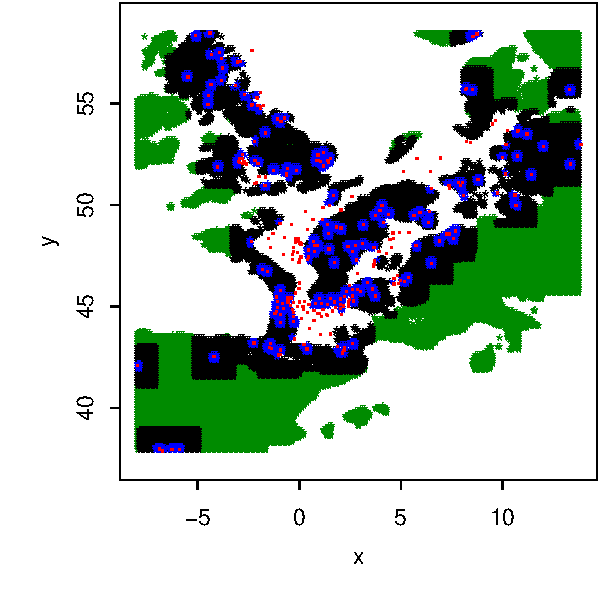
\includegraphics[width=\maxwidth]{figure/graphics-mopa8-1} 

}



\end{knitrout}

Function \texttt{PseudoAbsences} creates pseudo--absences either at random (TS method) or using the k-means clustering approach (TSKM method) for all the background extents considered. Prevalence (proportion of presences against pseudo--absences) and the exclusion buffer (minimum distance to be kept to presences without pseudo-absences) can also be set in this function using the arguments \texttt{prevalence} and \texttt{exclusion.buffer}.

\paragraph{At random (TS method)}

In the example below, pseudo--absences are generated at random, in equal number to presences (prevalence) and keeping a 10 km distance to presences (exclusion buffer).


\begin{knitrout}
\definecolor{shadecolor}{rgb}{0.965, 0.965, 0.965}\color{fgcolor}\begin{kframe}
\begin{alltt}
\hlstd{pa_random} \hlkwb{<-}\hlkwd{PseudoAbsences}\hlstd{(}\hlkwc{xy} \hlstd{= Oak_phylo2,} \hlkwc{bg.grids} \hlstd{= ext,}
                           \hlkwc{exclusion.buffer} \hlstd{=} \hlnum{0.083}\hlstd{,}
                           \hlkwc{prevalence} \hlstd{=} \hlnum{0.5}\hlstd{,} \hlkwc{kmeans} \hlstd{=} \hlnum{FALSE}\hlstd{)}
\end{alltt}
\begin{verbatim}
## [1] "generating pseudo-absences for species 1 out of 2"
## [1] "generating pseudo-absences for species 2 out of 2"
\end{verbatim}
\begin{alltt}
\hlcom{# Plot presences/pseudo-absences for group H11 considering the }
\hlcom{# background extent of 120 km}
\hlkwd{plot}\hlstd{(ext}\hlopt{$}\hlstd{H11}\hlopt{$}\hlstd{km120,} \hlkwc{pch}\hlstd{=}\hlstr{"*"}\hlstd{,} \hlkwc{col}\hlstd{=} \hlstr{"grey"}\hlstd{,} \hlkwc{cex}\hlstd{=}\hlnum{.5}\hlstd{,} \hlkwc{asp}\hlstd{=}\hlnum{1}\hlstd{)}
\hlkwd{points}\hlstd{(pa_random}\hlopt{$}\hlstd{H11}\hlopt{$}\hlstd{km120,} \hlkwc{col}\hlstd{=} \hlstr{"red"}\hlstd{,} \hlkwc{pch}\hlstd{=}\hlstr{"."}\hlstd{,} \hlkwc{cex}\hlstd{=}\hlnum{3}\hlstd{)}
\hlkwd{points}\hlstd{(Oak_phylo2}\hlopt{$}\hlstd{H11,} \hlkwc{col}\hlstd{=} \hlstr{"blue"}\hlstd{,} \hlkwc{pch}\hlstd{=}\hlstr{"."}\hlstd{,} \hlkwc{cex}\hlstd{=}\hlnum{3}\hlstd{)}
\end{alltt}
\end{kframe}

{\centering 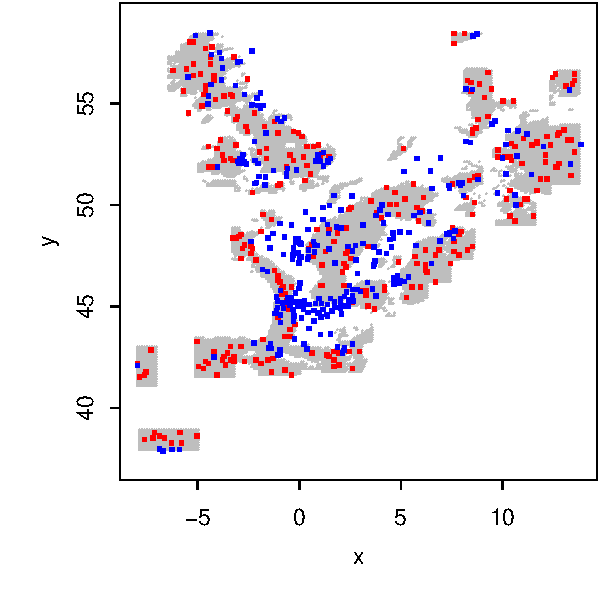
\includegraphics[width=\maxwidth]{figure/graphics-mopa9-1} 

}



\end{knitrout}

\paragraph{With k-means clustering (TSKM method)}

In the example below, pseudo-absences are generated with k-means clustering, in equal number to presences (prevalence) and keeping a 10 km distance to presences (exclusion buffer).

\begin{knitrout}
\definecolor{shadecolor}{rgb}{0.965, 0.965, 0.965}\color{fgcolor}\begin{kframe}
\begin{alltt}
\hlstd{pa_kmeans} \hlkwb{<-}\hlkwd{PseudoAbsences}\hlstd{(}\hlkwc{xy} \hlstd{= Oak_phylo2,} \hlkwc{bg.grids} \hlstd{= ext,}
                           \hlkwc{exclusion.buffer} \hlstd{=} \hlnum{0.083}\hlstd{,}
                           \hlkwc{prevalence} \hlstd{=} \hlnum{0.5}\hlstd{,} \hlkwc{kmeans} \hlstd{=} \hlnum{TRUE}\hlstd{,}
                           \hlkwc{varstack} \hlstd{= biostack)}
\end{alltt}
\begin{verbatim}
## [1] "generating pseudo-absences for species 1 out of 2"
## [1] "generating pseudo-absences for species 2 out of 2"
\end{verbatim}
\begin{alltt}
\hlcom{# Plot presences/pseudo-absences for group H11 considering }
\hlcom{# the background extent of 120 km}
\hlkwd{plot}\hlstd{(ext}\hlopt{$}\hlstd{H11}\hlopt{$}\hlstd{km120,} \hlkwc{pch} \hlstd{=} \hlstr{"*"}\hlstd{,} \hlkwc{col} \hlstd{=} \hlstr{"grey"}\hlstd{,} \hlkwc{cex} \hlstd{=} \hlnum{.5}\hlstd{,} \hlkwc{asp} \hlstd{=} \hlnum{1}\hlstd{)}
\hlkwd{points}\hlstd{(pa_kmeans}\hlopt{$}\hlstd{H11}\hlopt{$}\hlstd{km120,} \hlkwc{col} \hlstd{=} \hlstr{"red"}\hlstd{,} \hlkwc{pch} \hlstd{=} \hlstr{"."}\hlstd{,} \hlkwc{cex} \hlstd{=} \hlnum{3}\hlstd{)}
\hlkwd{points}\hlstd{(Oak_phylo2}\hlopt{$}\hlstd{H11,} \hlkwc{col} \hlstd{=} \hlstr{"blue"}\hlstd{,} \hlkwc{pch} \hlstd{=} \hlstr{"."}\hlstd{,} \hlkwc{cex} \hlstd{=} \hlnum{3}\hlstd{)}
\end{alltt}
\end{kframe}

{\centering 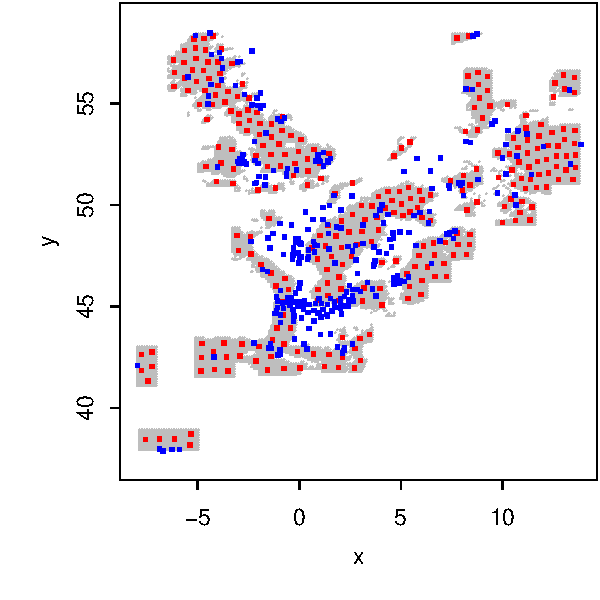
\includegraphics[width=\maxwidth]{figure/graphics-mopa10-1} 

}



\end{knitrout}


Function \texttt{bindPresAbs} binds presence and absence data for each background extension.

\begin{knitrout}
\definecolor{shadecolor}{rgb}{0.965, 0.965, 0.965}\color{fgcolor}\begin{kframe}
\begin{alltt}
\hlstd{presausTS} \hlkwb{<-} \hlkwd{bindPresAbs}\hlstd{(}\hlkwc{presences} \hlstd{= Oak_phylo2,}
                       \hlkwc{absences} \hlstd{= pa_random)}
\end{alltt}
\end{kframe}
\end{knitrout}

The \texttt{allModeling} function performs the species distribution modelling and the k-fold cross-validation for a set of presence/absence data per species, corresponding to different background 
extents. Algorithms supported are "glm", "svm", "maxent", "mars", "randomForest", "cart.rpart" 
and "cart.tree". In the example below, we perform a 10--fold cross validation using the "mars" modelling algorithm.


\begin{knitrout}
\definecolor{shadecolor}{rgb}{0.965, 0.965, 0.965}\color{fgcolor}\begin{kframe}
\begin{alltt}
\hlstd{modirsTS} \hlkwb{<-} \hlkwd{allModeling}\hlstd{(}\hlkwc{data} \hlstd{= presausTS,}
                     \hlkwc{varstack} \hlstd{= biostack,} \hlkwc{k} \hlstd{=} \hlnum{10}\hlstd{,}
                     \hlkwc{algorithm} \hlstd{=} \hlstr{"mars"}\hlstd{,} \hlkwc{destdir} \hlstd{=} \hlkwd{getwd}\hlstd{(),}
                \hlkwc{projection} \hlstd{=} \hlkwd{CRS}\hlstd{(}\hlstr{"+proj=longlat +init=epsg:4326"}\hlstd{))}
\end{alltt}
\end{kframe}
\end{knitrout}

Named .Rdata objects are stored in the specified directory in \texttt{destdir}. Each file is automatically named, indicating the algorithm, background extent, and species/population in this order (if a single species is provided, no name is given for the species). For instance, the file \textit{mars\_bgkm20\_hgH11.Rdata} stores the R object (a \texttt{list}) containing the SDM results for the MARS algorithm, considering a 20 km background extent and the Oak group H11. In particular, the output list contains the following components:

	(1)allmod: fitted model with all data for training, 
	(2)auc: AUC statistic in the cross validation,
	(3)kappa: kappa statistic in the cross validation,
	(4)tss: true skill statistic in the cross validation,
	(5)mod: fitted model with partitioned data, 
	(6)p: cross model prediction. 

\subsubsection{STEP3: selection of the optimum background extent and corresponding fitted model}

In the third step, AUCs obtained and corresponding extents are fitted to a Michaelis-Menten model to extract the \textit{Vm} coefficient (equation 1 in the manuscript). Then, the minimum extent at which the AUC surpasses the \textit{Vm} value is selected as the threshold extent (see Figure 3 in the manuscript), being the corresponding fitted SDM the definitive to predict suitability probabilities in the study area.

We next indicate how to plot the results of the optimal spatial extent selection using the \texttt{lattice} package. First we load the data generated with the \texttt{allModeling} function and extract the corresponding AUC values. Function \texttt{loadTestValues} loads and stores AUC data in a matrix:

\begin{knitrout}
\definecolor{shadecolor}{rgb}{0.965, 0.965, 0.965}\color{fgcolor}\begin{kframe}
\begin{alltt}
\hlstd{auc_mars} \hlkwb{<-}\hlkwd{loadTestValues}\hlstd{(}\hlkwc{data} \hlstd{= presausTS,} \hlkwc{test} \hlstd{=} \hlstr{"auc"}\hlstd{,}
                          \hlkwc{algorithm} \hlstd{=} \hlstr{"mars"}\hlstd{)}
\end{alltt}
\begin{verbatim}
## [1] "loading values for species 1"
## [1] "loading values for species 2"
\end{verbatim}
\begin{alltt}
\hlkwd{library}\hlstd{(lattice)}
\hlkwd{levelplot}\hlstd{(auc_mars,} \hlkwc{aspect} \hlstd{=} \hlnum{5}\hlstd{,}
          \hlkwc{scales} \hlstd{=} \hlkwd{list}\hlstd{(}\hlkwc{y} \hlstd{=} \hlkwd{list}\hlstd{(}\hlkwc{cex} \hlstd{=} \hlnum{0.8}\hlstd{,}
              \hlkwc{at} \hlstd{=} \hlkwd{c}\hlstd{(}\hlnum{1}\hlstd{,} \hlnum{49}\hlstd{,} \hlkwd{ncol}\hlstd{(auc_mars)),}
              \hlkwc{labels} \hlstd{=} \hlkwd{c}\hlstd{(}\hlkwd{colnames}\hlstd{(auc_mars)[}\hlnum{1}\hlstd{],}
                        \hlkwd{colnames}\hlstd{(auc_mars)[}\hlnum{49}\hlstd{],}
                        \hlkwd{colnames}\hlstd{(auc_mars)[}\hlkwd{ncol}\hlstd{(auc_mars)]))),}
          \hlkwc{at} \hlstd{=} \hlkwd{seq}\hlstd{(}\hlnum{0.6}\hlstd{,} \hlnum{1}\hlstd{,} \hlnum{0.01}\hlstd{),} \hlkwc{col.regions} \hlstd{= bpy.colors,}
          \hlkwc{xlab} \hlstd{=} \hlstr{"Haplogroups"}\hlstd{,} \hlkwc{ylab} \hlstd{=} \hlstr{"Background extent (km)"}\hlstd{,}
          \hlkwc{main} \hlstd{=} \hlstr{"AUC"}\hlstd{)}
\end{alltt}
\end{kframe}

{\centering 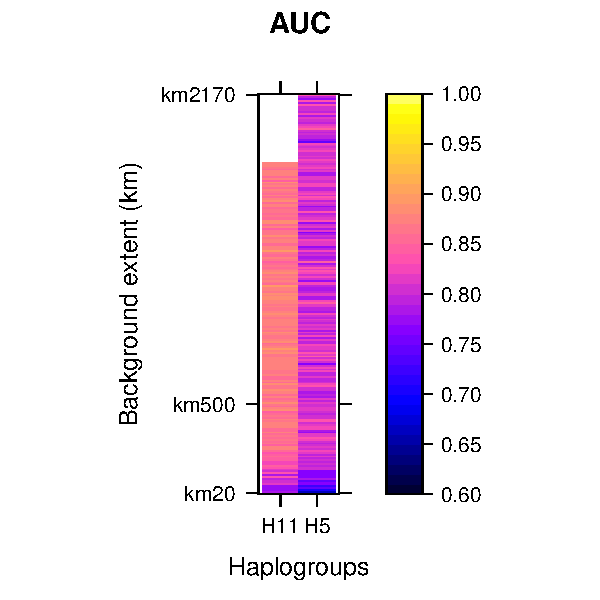
\includegraphics[width=\maxwidth]{figure/graphics-mopa13-1} 

}



\end{knitrout}


Model fitting is done by function \texttt{indextent}, that internally uses the \texttt{nls} function of R package \texttt{stats}. An index of the threshold extents is obtained. A fitted model plot (as in Fig. 3 in Iturbide et al., 2015) is also returned if argument \texttt{diagrams} is set to \texttt{TRUE}. 

\begin{knitrout}
\definecolor{shadecolor}{rgb}{0.965, 0.965, 0.965}\color{fgcolor}\begin{kframe}
\begin{alltt}
\hlstd{ind} \hlkwb{<-} \hlkwd{indextent}\hlstd{(}\hlkwc{testmat} \hlstd{= auc_mars,} \hlkwc{diagrams} \hlstd{=} \hlnum{TRUE}\hlstd{)}
\end{alltt}


{\ttfamily\noindent\itshape\color{messagecolor}{\#\# :::::::::::::::::::::::::::::::::::::::::::::::::::::::::::::::::::::::::::::\\\#\# residual sum of squares for species\ \ H11\\\#\# exponential3 = 0.0185340230599441\\\#\# Michaelis Menten = 0.0261508567502973\\\#\# exponential2 = 0.0696316706281794\\\#\# best function =\ \ exponential3\\\#\# :::::::::::::::::::::::::::::::::::::::::::::::::::::::::::::::::::::::::::::\\\#\# residual sum of squares for species\ \ H5\\\#\# exponential3 = 0.0628713268171315\\\#\# Michaelis Menten = 0.0676137627133294\\\#\# exponential2 = 0.0909438802483496\\\#\# best function =\ \ exponential3\\\#\# :::::::::::::::::::::::::::::::::::::::::::::::::::::::::::::::::::::::::::::}}\begin{alltt}
\hlstd{ind}
\end{alltt}
\begin{verbatim}
## km270 km160 
##    26    15
\end{verbatim}
\end{kframe}

{\centering 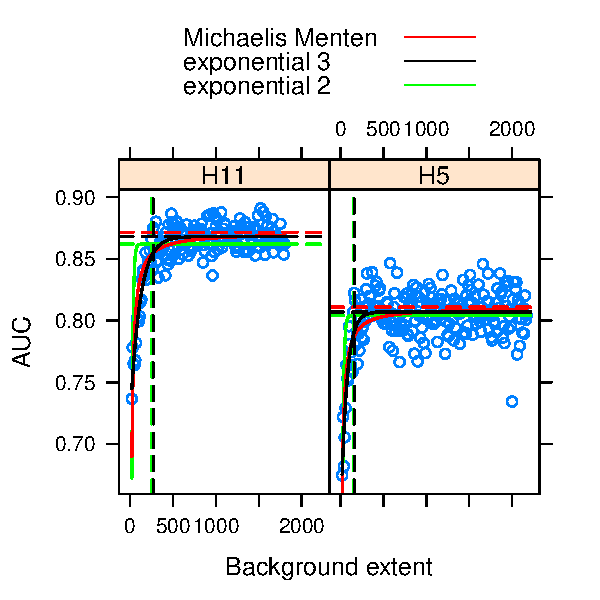
\includegraphics[width=\maxwidth]{figure/graphics-mopa14-1} 

}



\end{knitrout}

The \texttt{ind} object in the example above gives the index to extract the best model components and associated data, by means of function \texttt{loadDefinitiveModel}.  

\begin{knitrout}
\definecolor{shadecolor}{rgb}{0.965, 0.965, 0.965}\color{fgcolor}\begin{kframe}
\begin{alltt}
\hlstd{def} \hlkwb{<-}\hlkwd{loadDefinitiveModel}\hlstd{(}\hlkwc{data} \hlstd{= presausTS,}
              \hlkwc{extents} \hlstd{= ind,} \hlkwc{slot} \hlstd{=} \hlstr{"allmod"}\hlstd{,} \hlkwc{algorithm} \hlstd{=} \hlstr{"mars"}\hlstd{)}
\end{alltt}
\end{kframe}
\end{knitrout}

Once the optimal SDMs are chosen, we can generate the resulting suitability maps. In the example below we use function \texttt{biomat} for preparing a matrix with the variables for prediction in the study area. Then, the predictions are converted to a raster format with functions \texttt{SpatialPixelsDataFrame} (from the \texttt{sp} package) and \texttt{raster} (from the \texttt{raster} package).

\begin{knitrout}
\definecolor{shadecolor}{rgb}{0.965, 0.965, 0.965}\color{fgcolor}\begin{kframe}
\begin{alltt}
\hlcom{# Suitability map for the Oak group H11}
\hlcom{# Function 'biomat' prepares matrix with variables for projection}
\hlstd{projectionland} \hlkwb{<-} \hlkwd{biomat}\hlstd{(}\hlkwd{cbind}\hlstd{(box.grid}\hlopt{$}\hlstd{bbs.grid}\hlopt{$}\hlstd{H11,}
                        \hlkwd{rep}\hlstd{(}\hlnum{1}\hlstd{,} \hlkwd{nrow}\hlstd{(box.grid}\hlopt{$}\hlstd{bbs.grid}\hlopt{$}\hlstd{H11))),}
                         \hlstd{biostack)}
\hlcom{# Prediction}
\hlstd{p} \hlkwb{<-} \hlkwd{predict}\hlstd{(def}\hlopt{$}\hlstd{H11, projectionland[ ,}\hlopt{-}\hlnum{1}\hlstd{])}
\hlstd{p[}\hlkwd{which}\hlstd{(p} \hlopt{<} \hlnum{0}\hlstd{)]} \hlkwb{<-} \hlnum{0}
\hlstd{p[}\hlkwd{which}\hlstd{(p} \hlopt{>} \hlnum{1}\hlstd{)]} \hlkwb{<-} \hlnum{1}
\hlcom{# Convert prediction to a raster object}
\hlstd{spp} \hlkwb{<-} \hlkwd{SpatialPixelsDataFrame}\hlstd{(box.grid}\hlopt{$}\hlstd{bbs.grid}\hlopt{$}\hlstd{H11,}
                              \hlkwd{as.data.frame}\hlstd{(p))}
\hlstd{ras} \hlkwb{<-} \hlkwd{raster}\hlstd{(spp)}
\hlkwd{plot}\hlstd{(ras)}
\end{alltt}
\end{kframe}

{\centering 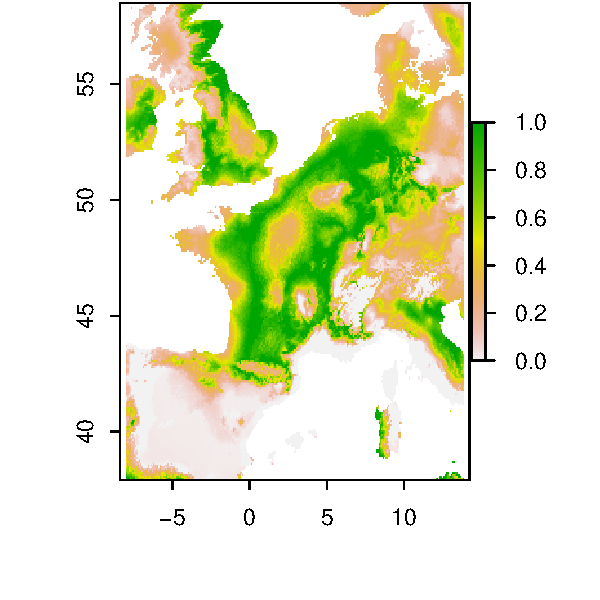
\includegraphics[width=\maxwidth]{figure/graphics-mopa16-1} 

}



\end{knitrout}



%unsrtnat
% \bibliographystyle{elsarticle-harv}
% \bibliography{gen2}

We can combine functions in \texttt{mopa} to apply alternative methods of pseudo-absence data generation. 
Functions performing each step in RSEP, TS and TSKM are indicated in the conceptual diagram of the manuscript (Fig. 2). Functions involved in the TS and TSKM methods are:\\

  \texttt{boundingCoords + delimit + OCSVMprofiling + bgRadio + \\
  pseudoAbsences + bindPresAbs + allModeling + loadTestValues +\\
  indextent + loadDefinitiveModel},\\  

while the RSEP method only applies the first step of the Three-step methods, being the involved functions:\\

  \texttt{boundingCoords + delimit + OCSVMprofiling + \\
  pseudoAbsences + allModeling}. \\
 
If we want to establish a threshold distance of the background but are not interested in doing an environmental profiling of the background in the previous step, we can combine functions this way:\\

  \texttt{boundingCoords + delimit + bgRadio + pseudoAbsences +\\ 
  bindPresAbs + allModeling + loadTestValues + indextent +\\
  loadDefinitiveModel}.


\begin{knitrout}
\definecolor{shadecolor}{rgb}{0.965, 0.965, 0.965}\color{fgcolor}\begin{kframe}
\begin{alltt}
\hlkwd{print}\hlstd{(}\hlkwd{sessionInfo}\hlstd{())}
\end{alltt}
\begin{verbatim}
## R version 3.2.0 (2015-04-16)
## Platform: x86_64-pc-linux-gnu (64-bit)
## Running under: Ubuntu 14.04.2 LTS
## 
## locale:
##  [1] LC_CTYPE=en_US.UTF-8      
##  [2] LC_NUMERIC=C              
##  [3] LC_TIME=es_ES.UTF-8       
##  [4] LC_COLLATE=en_US.UTF-8    
##  [5] LC_MONETARY=es_ES.UTF-8   
##  [6] LC_MESSAGES=en_US.UTF-8   
##  [7] LC_PAPER=es_ES.UTF-8      
##  [8] LC_NAME=C                 
##  [9] LC_ADDRESS=C              
## [10] LC_TELEPHONE=C            
## [11] LC_MEASUREMENT=es_ES.UTF-8
## [12] LC_IDENTIFICATION=C       
## 
## attached base packages:
## [1] stats     graphics  grDevices utils    
## [5] datasets  methods   base     
## 
## other attached packages:
## [1] lattice_0.20-31 mopa_0.2.0     
## [3] raster_2.3-40   sp_1.1-0       
## [5] devtools_1.8.0  knitr_1.10.5   
## 
## loaded via a namespace (and not attached):
##  [1] formatR_1.2           git2r_0.10.1         
##  [3] highr_0.5             TeachingDemos_2.9    
##  [5] bitops_1.0-6          class_7.3-12         
##  [7] tools_3.2.0           rpart_4.1-9          
##  [9] digest_0.6.8          goftest_1.0-2        
## [11] nlme_3.1-120          evaluate_0.7         
## [13] memoise_0.2.1         PresenceAbsence_1.1.9
## [15] mgcv_1.8-6            Matrix_1.2-0         
## [17] rgdal_0.9-3           spam_1.0-1           
## [19] dismo_1.0-12          e1071_1.6-4          
## [21] stringr_1.0.0         rversions_1.0.0      
## [23] grid_3.2.0            tree_1.0-35          
## [25] sampling_2.6          plotrix_3.5-12       
## [27] tcltk_3.2.0           XML_3.98-1.2         
## [29] plotmo_3.1.1          polyclip_1.3-2       
## [31] tensor_1.5            deldir_0.1-9         
## [33] magrittr_1.5          splancs_2.01-37      
## [35] codetools_0.2-11      MASS_7.3-39          
## [37] abind_1.4-3           randomForest_4.6-10  
## [39] spatstat_1.42-0       lpSolve_5.6.11       
## [41] earth_4.4.0           stringi_0.4-1        
## [43] RCurl_1.95-4.6
\end{verbatim}
\end{kframe}
\end{knitrout}


\section{References}

Iturbide, M., Bedia, J., Herrera, S., del Hierro, O., Pinto, M., Gutiérrez, J.M., 2015. A framework for
species distribution modelling with improved pseudo-absence generation. Ecological Modelling DOI:10.1016/j.ecolmodel.2015.05.018.


Petit, R. J., Csaikl, U. M., Bordács, S., Burg, K., Coart, E., Cottrell,J., van Dam, B., Deans, J. D., Dumolin-Lapégue, S., Fineschi, S., Finkeldey, R., Gillies, A., Glaz, I., Goicoechea, P. G., Jensen,J. S., König, A. O., Lowe, A. J., Madsen, S. F., Mátyás, G., Munro, R. C., Olalde, M., Pemonge, M.-H., Popescu, F., Slade, D., Tabbener, H., Taurchini, D., de Vries, S. G. M., Ziegenhagen, B., Kremer, A., 2002b. Chloroplast DNA variation in european white oaks: Phylogeography and patterns of diversity based on data from over 2600 populations. Forest Ecology and Management 156 (1–3), 5–26.

\end{document}


